\documentclass[a4paper,12pt]{article} 
\usepackage[top = 2cm, bottom = 1.5cm, left = 1.5cm, right = 1.5cm]{geometry} 
\usepackage[T1]{fontenc}
\usepackage[utf8]{inputenc}
\usepackage{booktabs} % For even nicer tables.
\usepackage{graphicx} 
\usepackage{setspace}
\setlength{\parindent}{0in}
\usepackage{float}

% The fancyhdr package let's us create nice headers.
\usepackage{fancyhdr}
\usepackage{amsmath,amsthm,amssymb}
\usepackage{enumitem}
\usepackage{subfig}
\usepackage{tikz}
%%%%%%%%%%%%%%%%%%%%%%%%%%%%%%%%%%%%%%%%%%%%%%%%
% 3. Header (and Footer)
%%%%%%%%%%%%%%%%%%%%%%%%%%%%%%%%%%%%%%%%%%%%%%%%
\pagestyle{fancy} % With this command we can customize the header style.
\fancyhf{} % This makes sure we do not have other information in our header or footer.
%% \lhead{\footnotesize }% \lhead puts text in the top left corner.
%% \footnotesize sets our font to a smaller size.
\chead{ \footnotesize Calculus Problem Set}
%\rhead works just like \lhead (you can also use \chead)
%\rhead{\footnotesize Lastname 1, Lastname 2 (\& Lastname 3)} %<---- Fill in your lastnames.

% Similar commands work for the footer (\lfoot, \cfoot and \rfoot).
% We want to put our page number in the center.
\cfoot{\footnotesize \thepage} 


%%%%%%%%%%%%%%%%%%%%%%%%%%%%%%%%%%%%%%%%%%%%%%%%
% 4. Your document
%%%%%%%%%%%%%%%%%%%%%%%%%%%%%%%%%%%%%%%%%%%%%%%%

% Now, you need to tell LaTeX where your document starts. We do this with the \begin{document} command.
% Like brackets every \begin{} command needs a corresponding \end{} command. We come back to this later.

\begin{document}


%%%%%%%%%%%%%%%%%%%%%%%%%%%%%%%%%%%%%%%%%%%%%%%%
%%%%%%%%%%%%%%%%%%%%%%%%%%%%%%%%%%%%%%%%%%%%%%%%

%%%%%%%%%%%%%%%%%%%%%%%%%%%%%%%%%%%%%%%%%%%%%%%%
% Title section of the document
%%%%%%%%%%%%%%%%%%%%%%%%%%%%%%%%%%%%%%%%%%%%%%%%

% For the title section we want to reproduce the title section of the Problem Set and add your names.

\thispagestyle{empty} % This command disables the header on the first page. 

\begin{center} % This is a simple tabular environment to align your text nicely 
{\Large \bf Calculus Problem Set} \\ \vspace{0.3cm}
\end{center} % Our tabular environment ends here.
%\newline

\vspace{-0.cm}
\rule{\textwidth}{2pt}
%%%%%%%%%%%%%%%%%%%%%%%%%%%%%%%%%%%%%%%%%%%%%%%%
%%%%%%%%%%%%%%%%%%%%%%%%%%%%%%%%%%%%%%%%%%%%%%%%
\vspace{-0.5cm}
\section*{\centering Direct}
\subsection*{Chain Derivative}
\begin{enumerate}
\item Find the derivative of $\tan(5-\sin 2t)$.
\end{enumerate}
\subsection*{Implict Derivative}
\begin{enumerate}
\item Find the derivative of $y^2 = x^2 + \sin(xy)$.
\end{enumerate}
\section*{\centering Applied}
\begin{enumerate}
  \item Water is being fed to cylinder of height $H$ and radius $R$ at a certain flow rate $Q$. Relate $Q$ with the liquid height $h$.
  
  \item Profile of an axisymmetric bowl is given by $z = ax^3$. While the total height of the bowl is 6 cm, it is filled only up to a height of 5 cm. (a) Find the volume of the liquid inside the cup. (b) How much can you tilt the cup before the liquid starts spilling?
  
 \begin{figure}[h]
 \begin{center}
 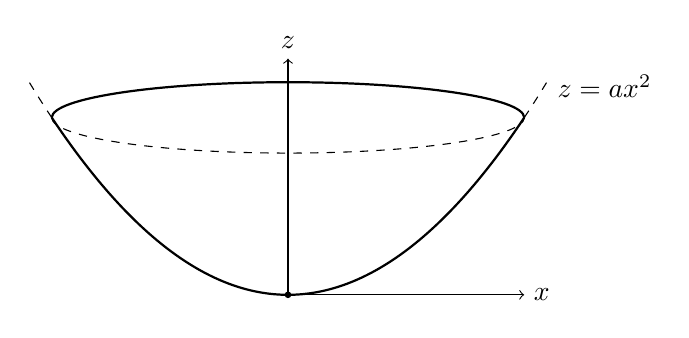
\begin{tikzpicture}[scale=1]

% Parameters
\def\a{0.25}    % z = a x^2
\def\R{3}        % rim radius
\pgfmathsetmacro{\H}{\a*\R*\R}

% Axis
\draw[->] (0,0) -- (0,3) node[above] {$z$};
\draw[->] (0,0) -- (3,0) node[right] {$x$};

% Front half of the cup
\draw[thick,domain=0:\R,samples=100]
      plot ({\x},{\a*\x*\x});
\draw[dashed,domain=\R:1.1*\R,samples=100]
      plot ({\x},{\a*\x*\x});

% Back half (symmetric)
\draw[thick,domain=0:\R,samples=100]
      plot ({-\x},{\a*\x*\x});
\draw[dashed,domain=\R:1.1*\R,samples=100]
      plot ({-\x},{\a*\x*\x});

% Bottom point
\fill (0,0) circle (1.2pt);

% Rim (ellipse to suggest revolution)
%\draw[thick] (0,\H) ellipse ({\R} and {0.45});
\draw[thick] (\R,\H) arc (0:180:{\R} and 0.45);

% Hidden back part of the rim
\draw[dashed] (-\R,\H) arc (180:360:{\R} and 0.45);

% Label
\node[right] at (1.1*\R,\H+0.4) {$z=ax^2$};

\end{tikzpicture}
\end{center}
 \caption{Axisymmetric cup with a profile of $z=ax^2$.}
\end{figure}
  
  \end{enumerate}
\end{document}
